\section{实验结果与分析}
经历综合实现,我们可以在开发板上看到测试的结果
我们分以下几个部分验证实验结果的正确性
\subsection{ALU与ls指令的forwarding和stall}
forwarding后紧接着需要用到读入的寄存器的alu指令时,需要在stall之后再进行forwarding。在图4.7中,load指令后紧接了一条ALU指令,因此我们在load指令后插入了一个stall,之后再进行forwarding操作。
\begin{figure}
	\centering %图片居中
	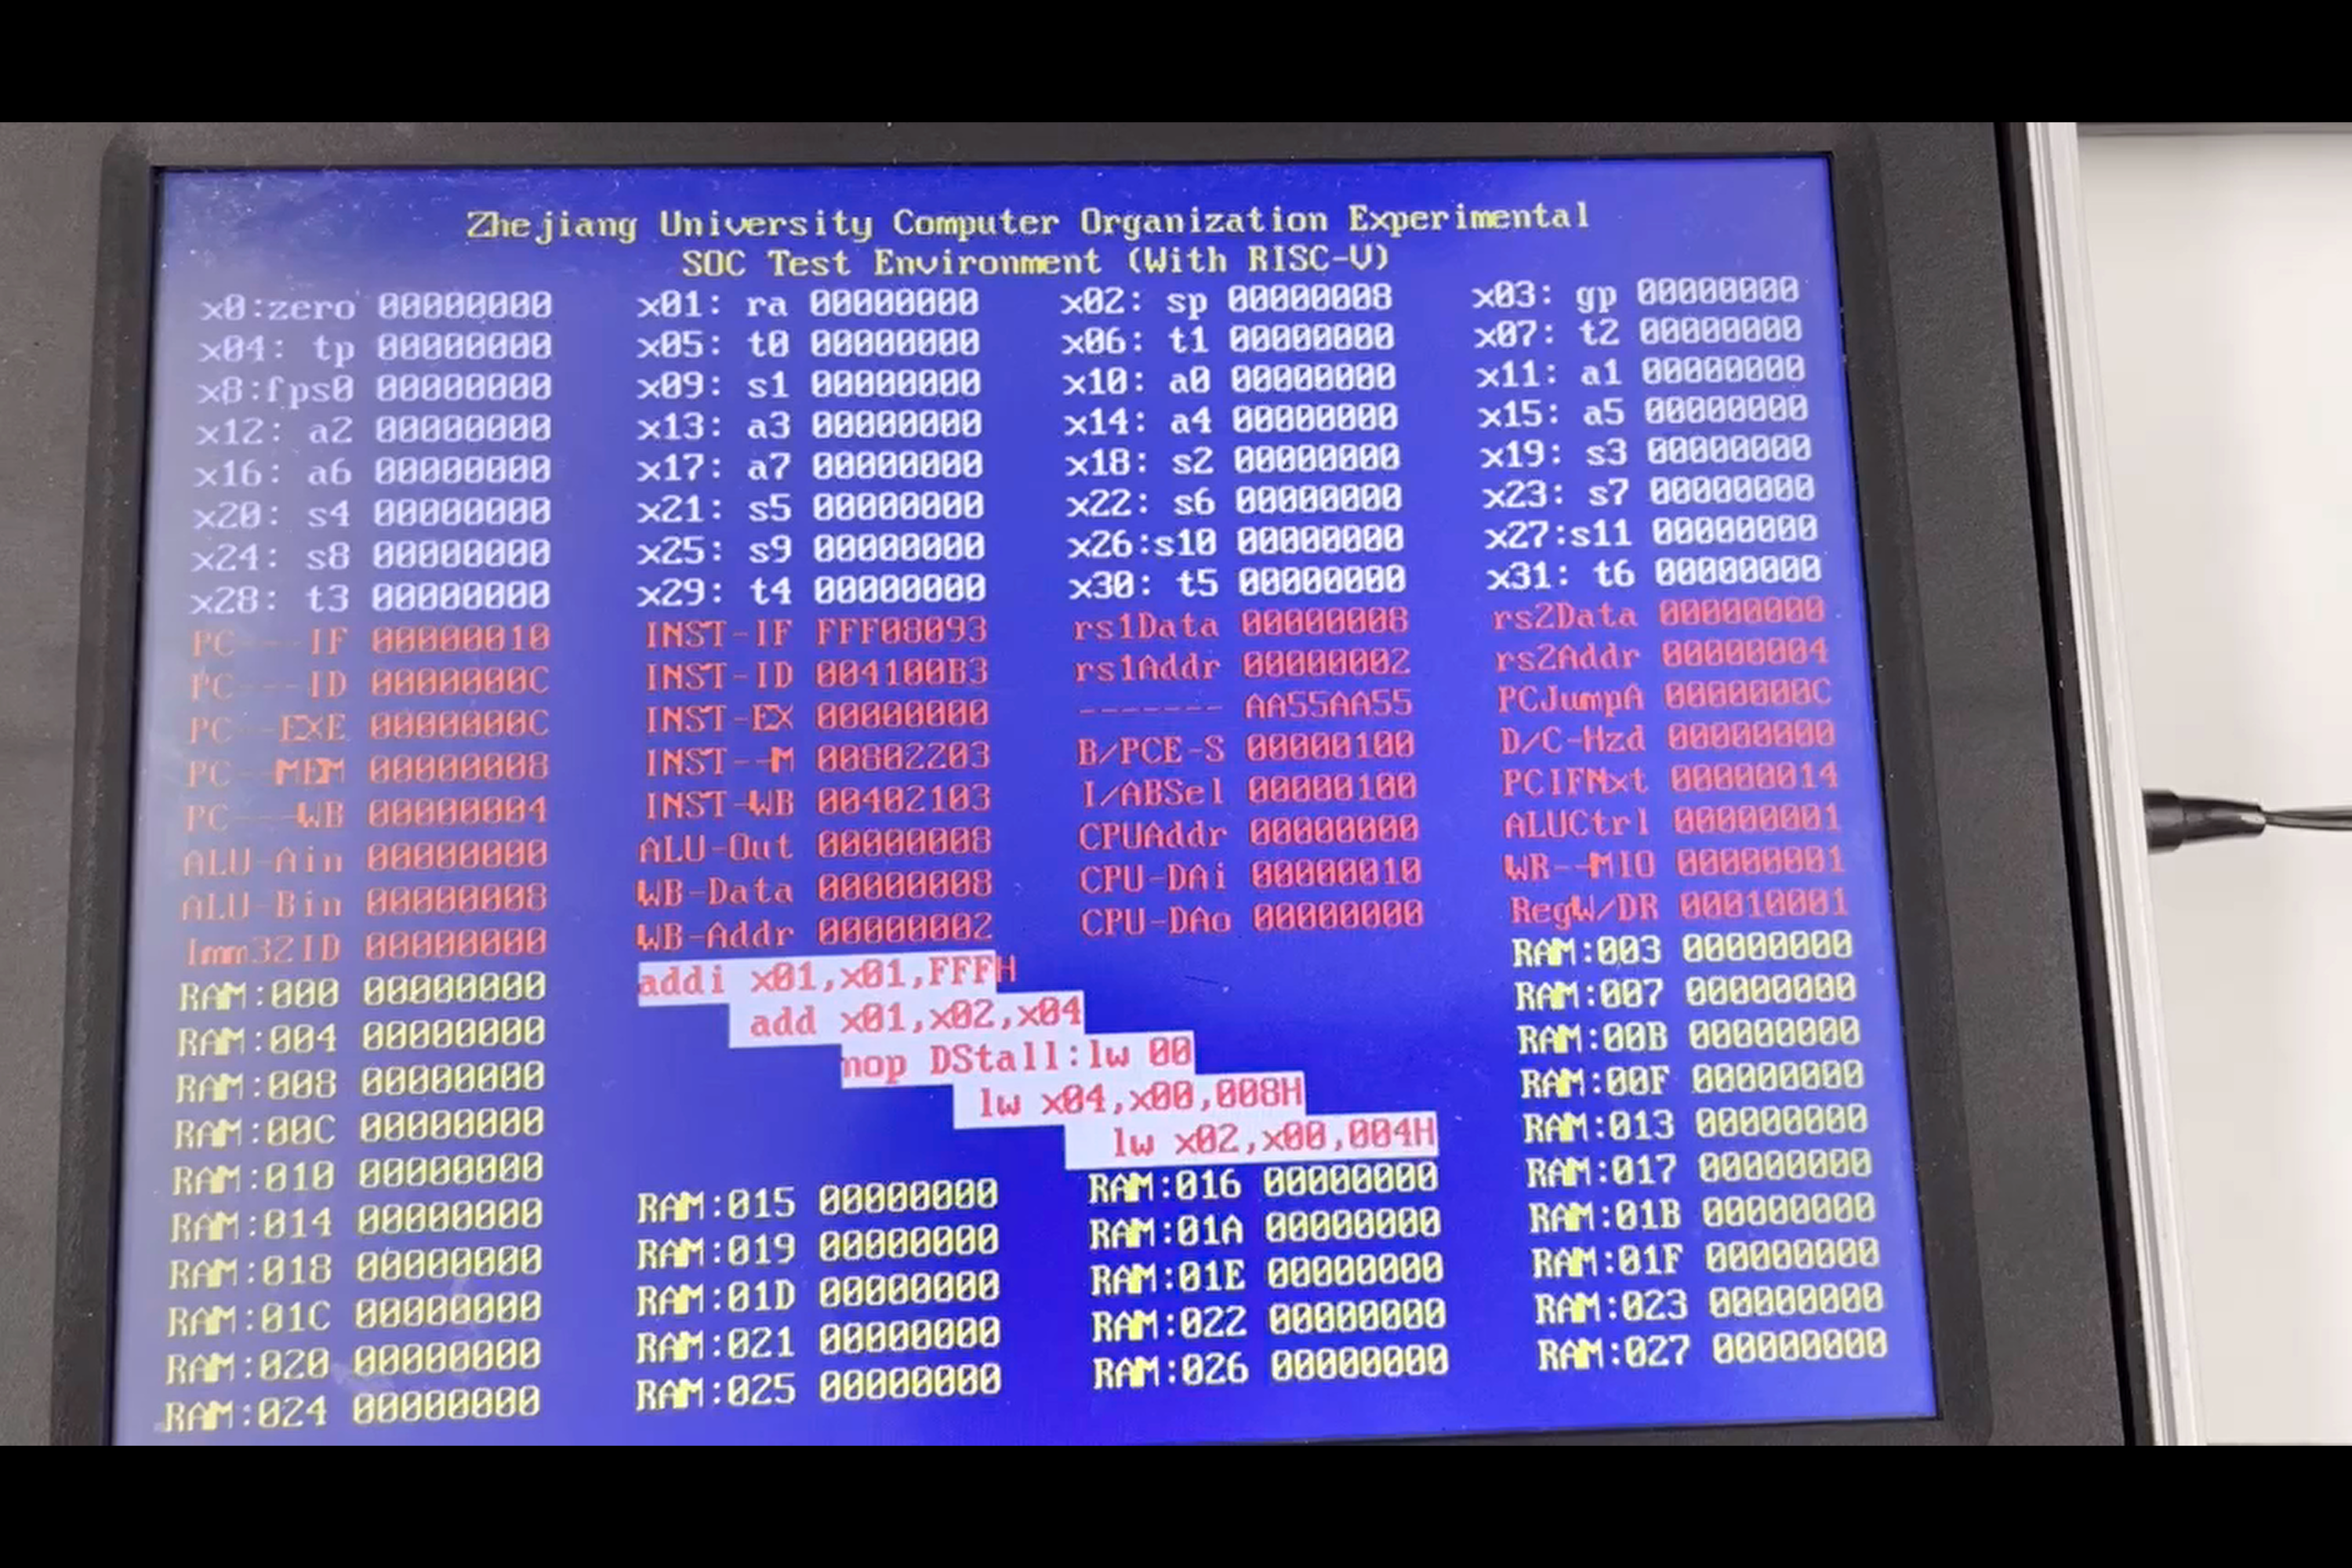
\includegraphics[width=1.0\textwidth]{y1.png} %插入图片,[]中设置图片大小,{}中是图片文件名
	\caption{验证结果图} %最终文档中希望显示的图片标题
	\label{Fig.7} %用于文内引用的标签
\end{figure}
\subsection{ALU指令检验}
之后时一长串正常的ALU指令,通过检测寄存器数值,确定运行结果正确,见图4.8
\begin{figure}
	\centering %图片居中
	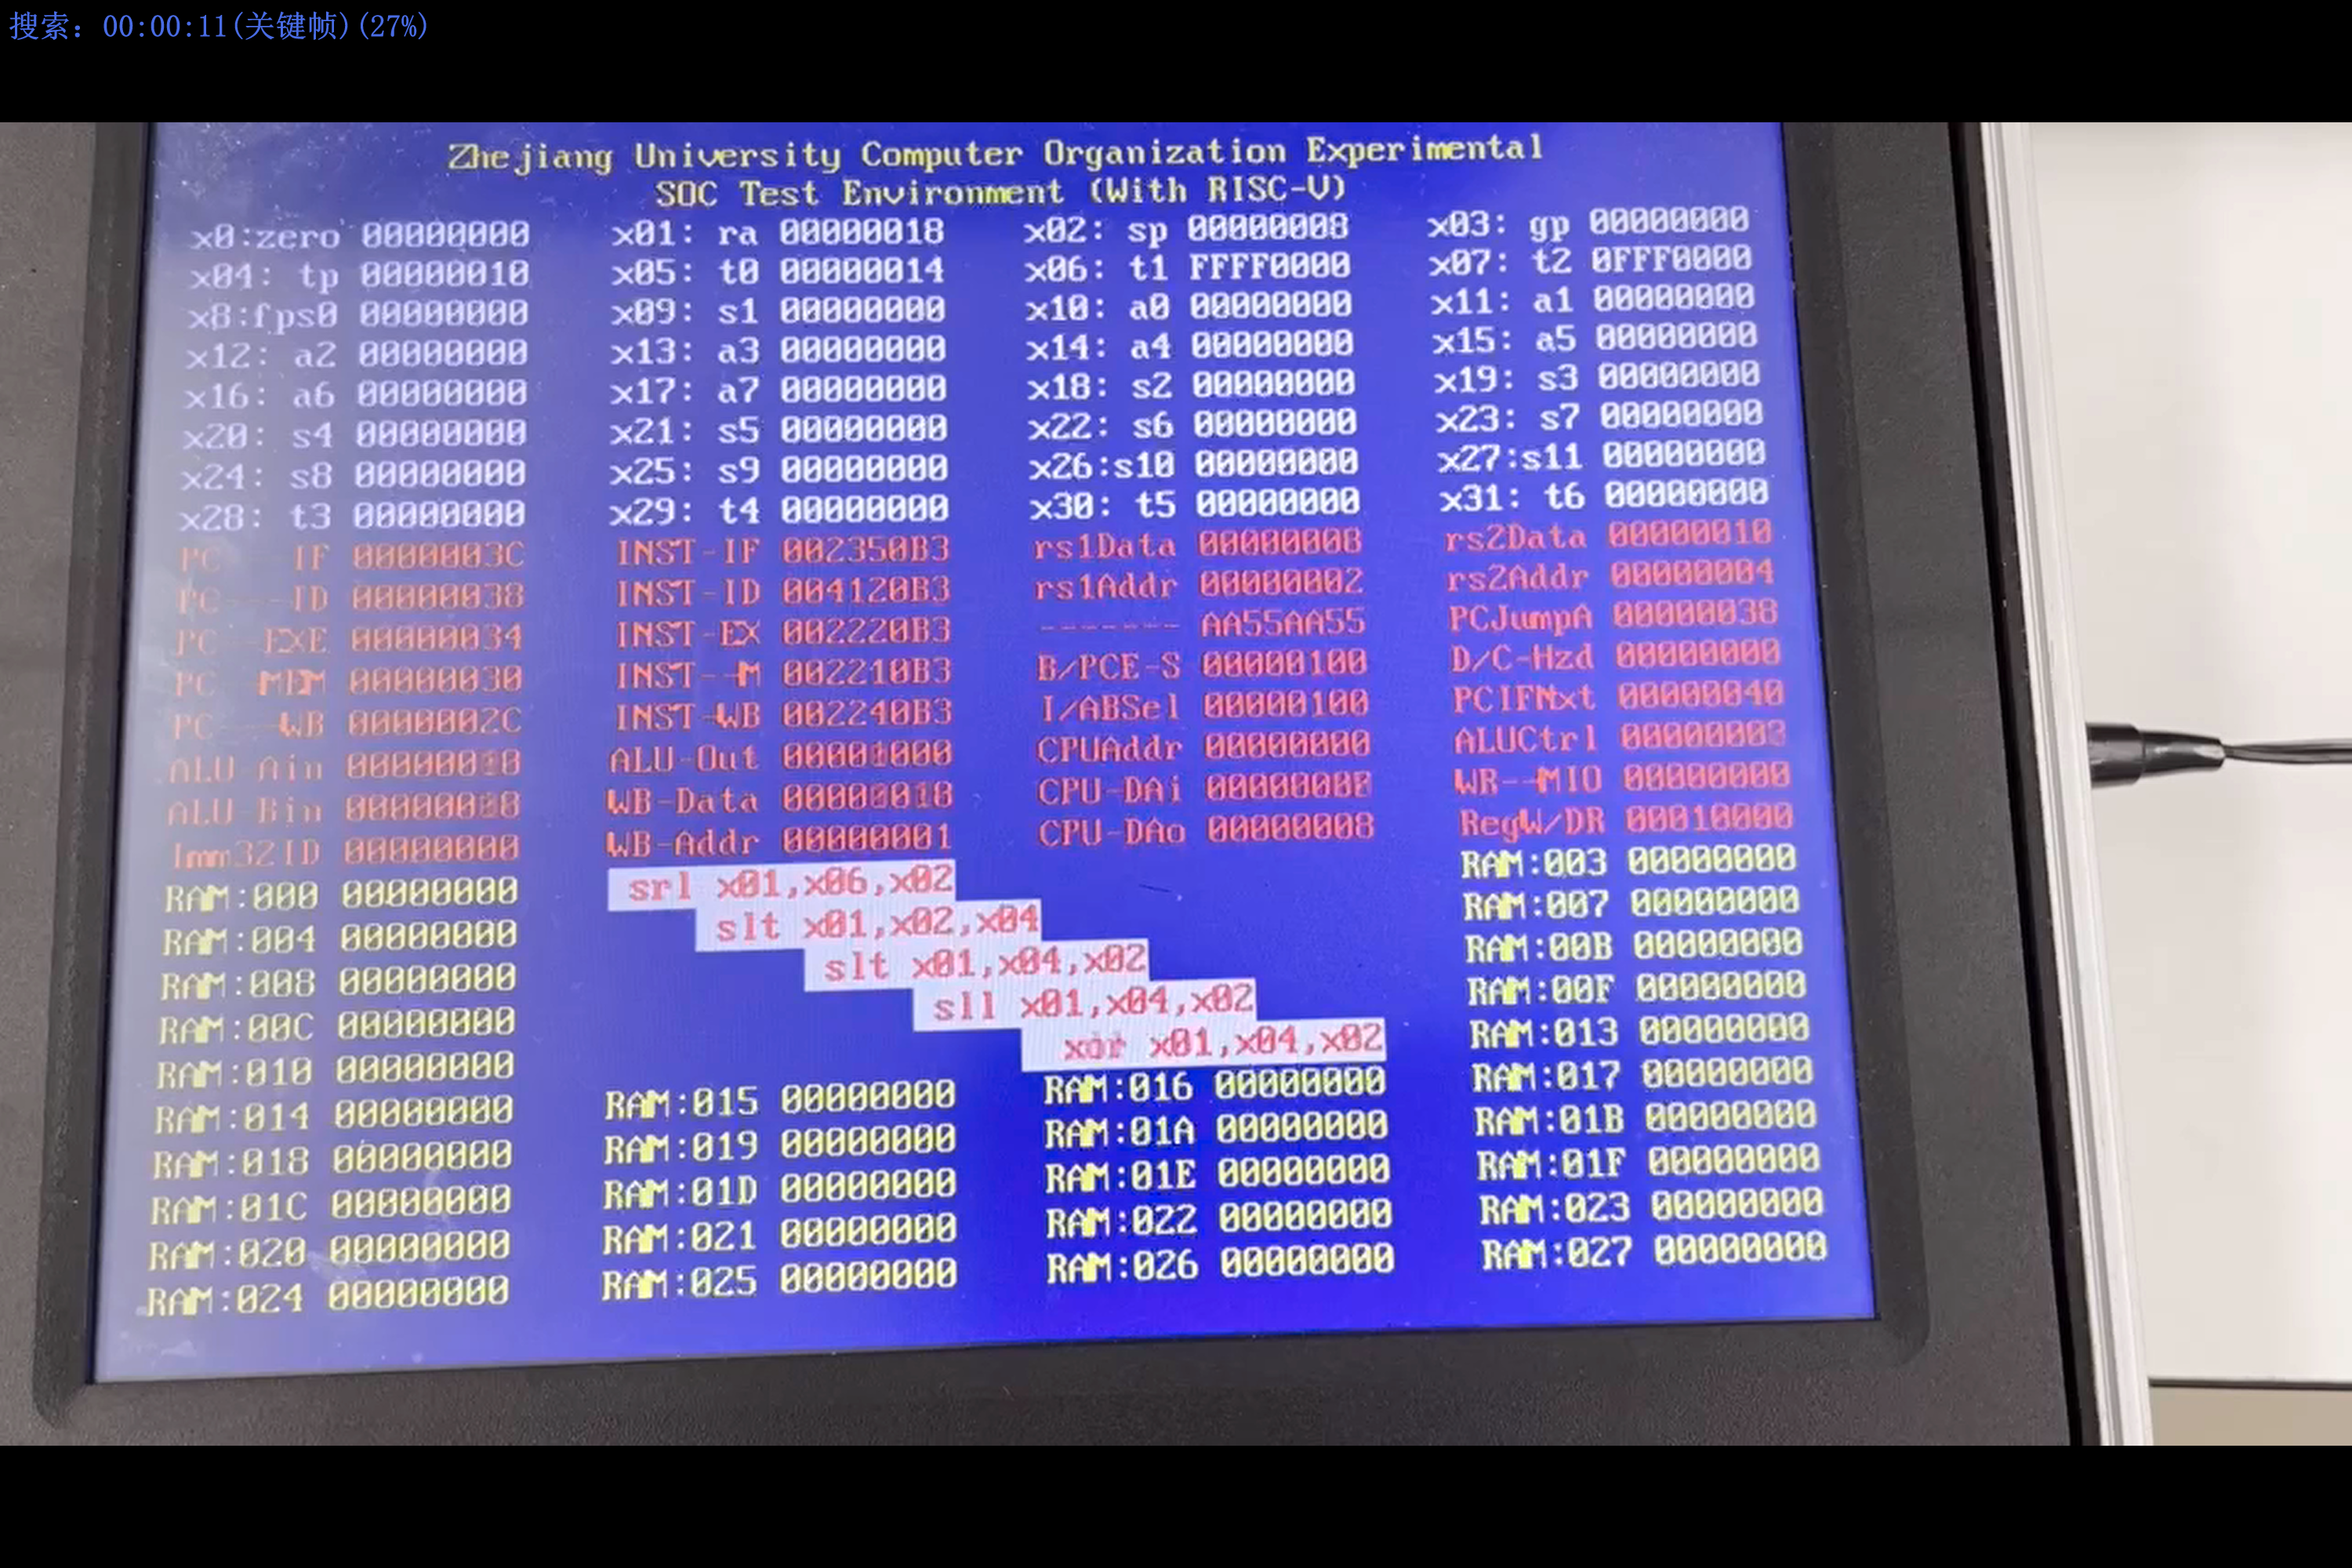
\includegraphics[width=1.0\textwidth]{y2.png} %插入图片,[]中设置图片大小,{}中是图片文件名
	\caption{验证结果图} %最终文档中希望显示的图片标题
	\label{Fig.8} %用于文内引用的标签
\end{figure}
\subsection{branch指令检验}
之后进入branch阶段,我们的branch再ID阶段实现,并且使用predict not taken,当需要跳转时,会删除已经读取的指令并插入一个stall。见图4.9
\begin{figure}
	\centering %图片居中
	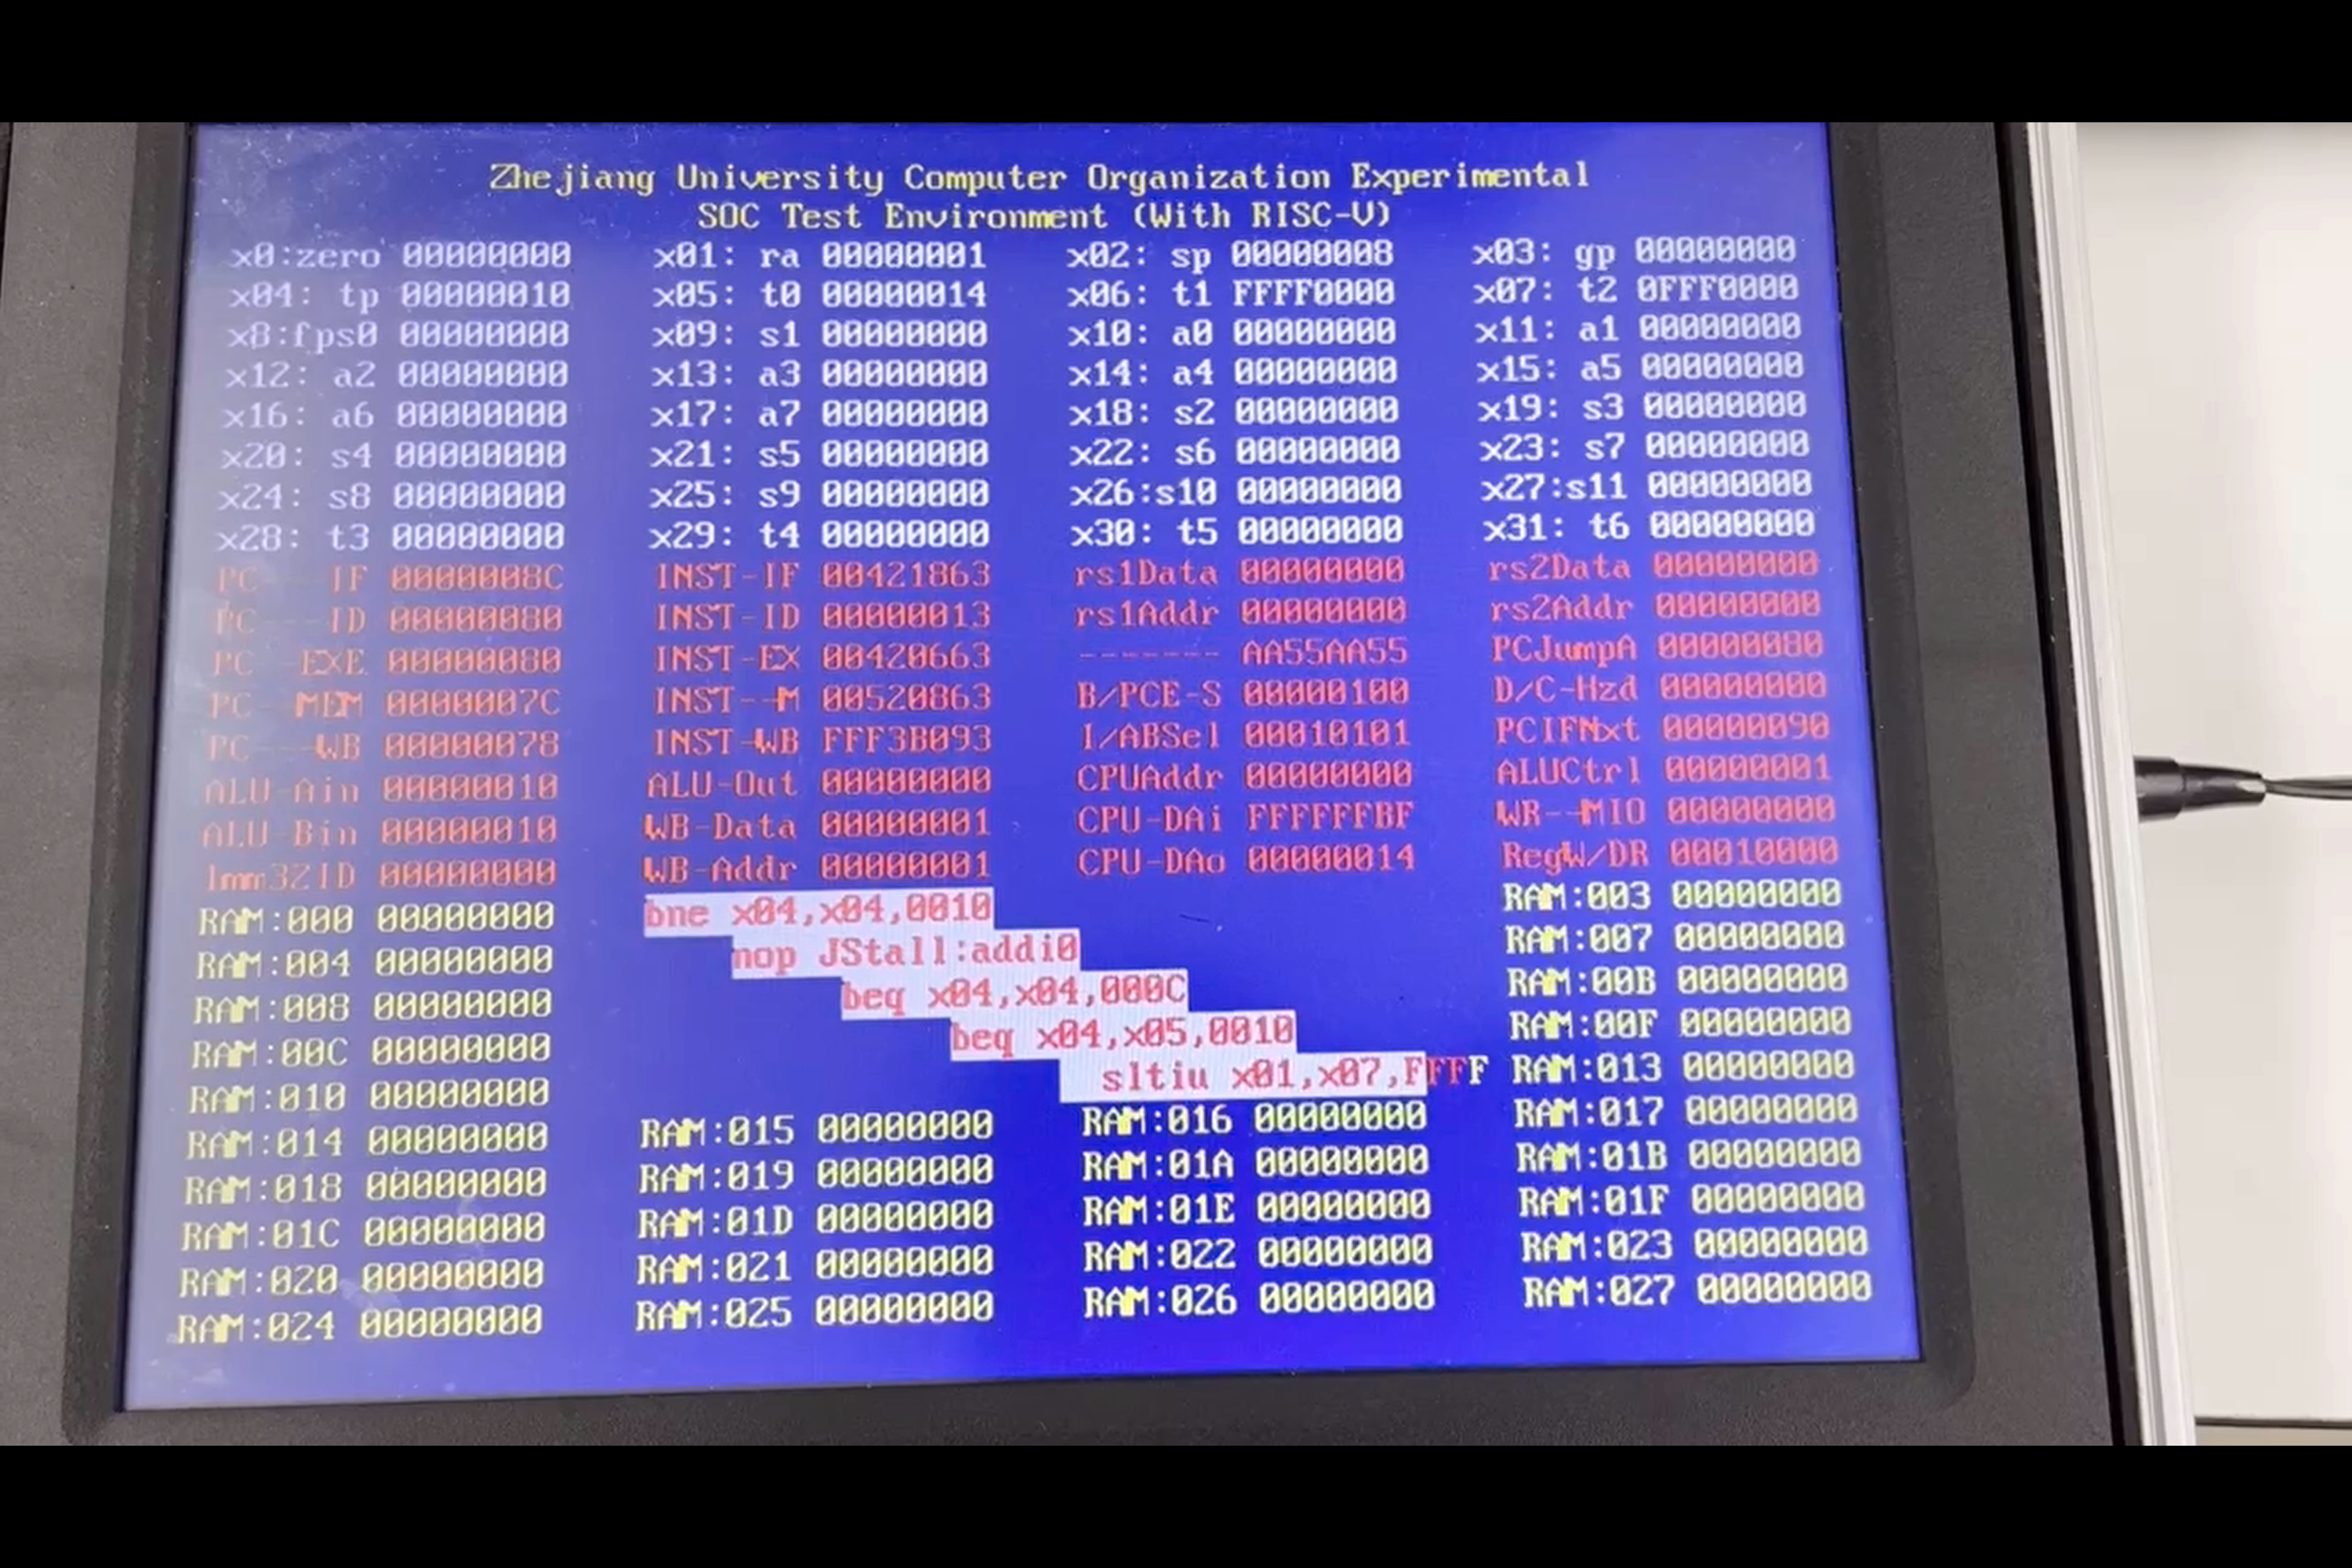
\includegraphics[width=1.0\textwidth]{y3.png} %插入图片,[]中设置图片大小,{}中是图片文件名
	\caption{验证结果图} %最终文档中希望显示的图片标题
	\label{Fig.9} %用于文内引用的标签
\end{figure}
\subsection{ls指令、lui、auipc指令}
之后是一系列load,store,lui,auipc等指令,经检验,运行结果正确。见图4.10、4.11
\begin{figure}
	\centering %图片居中
	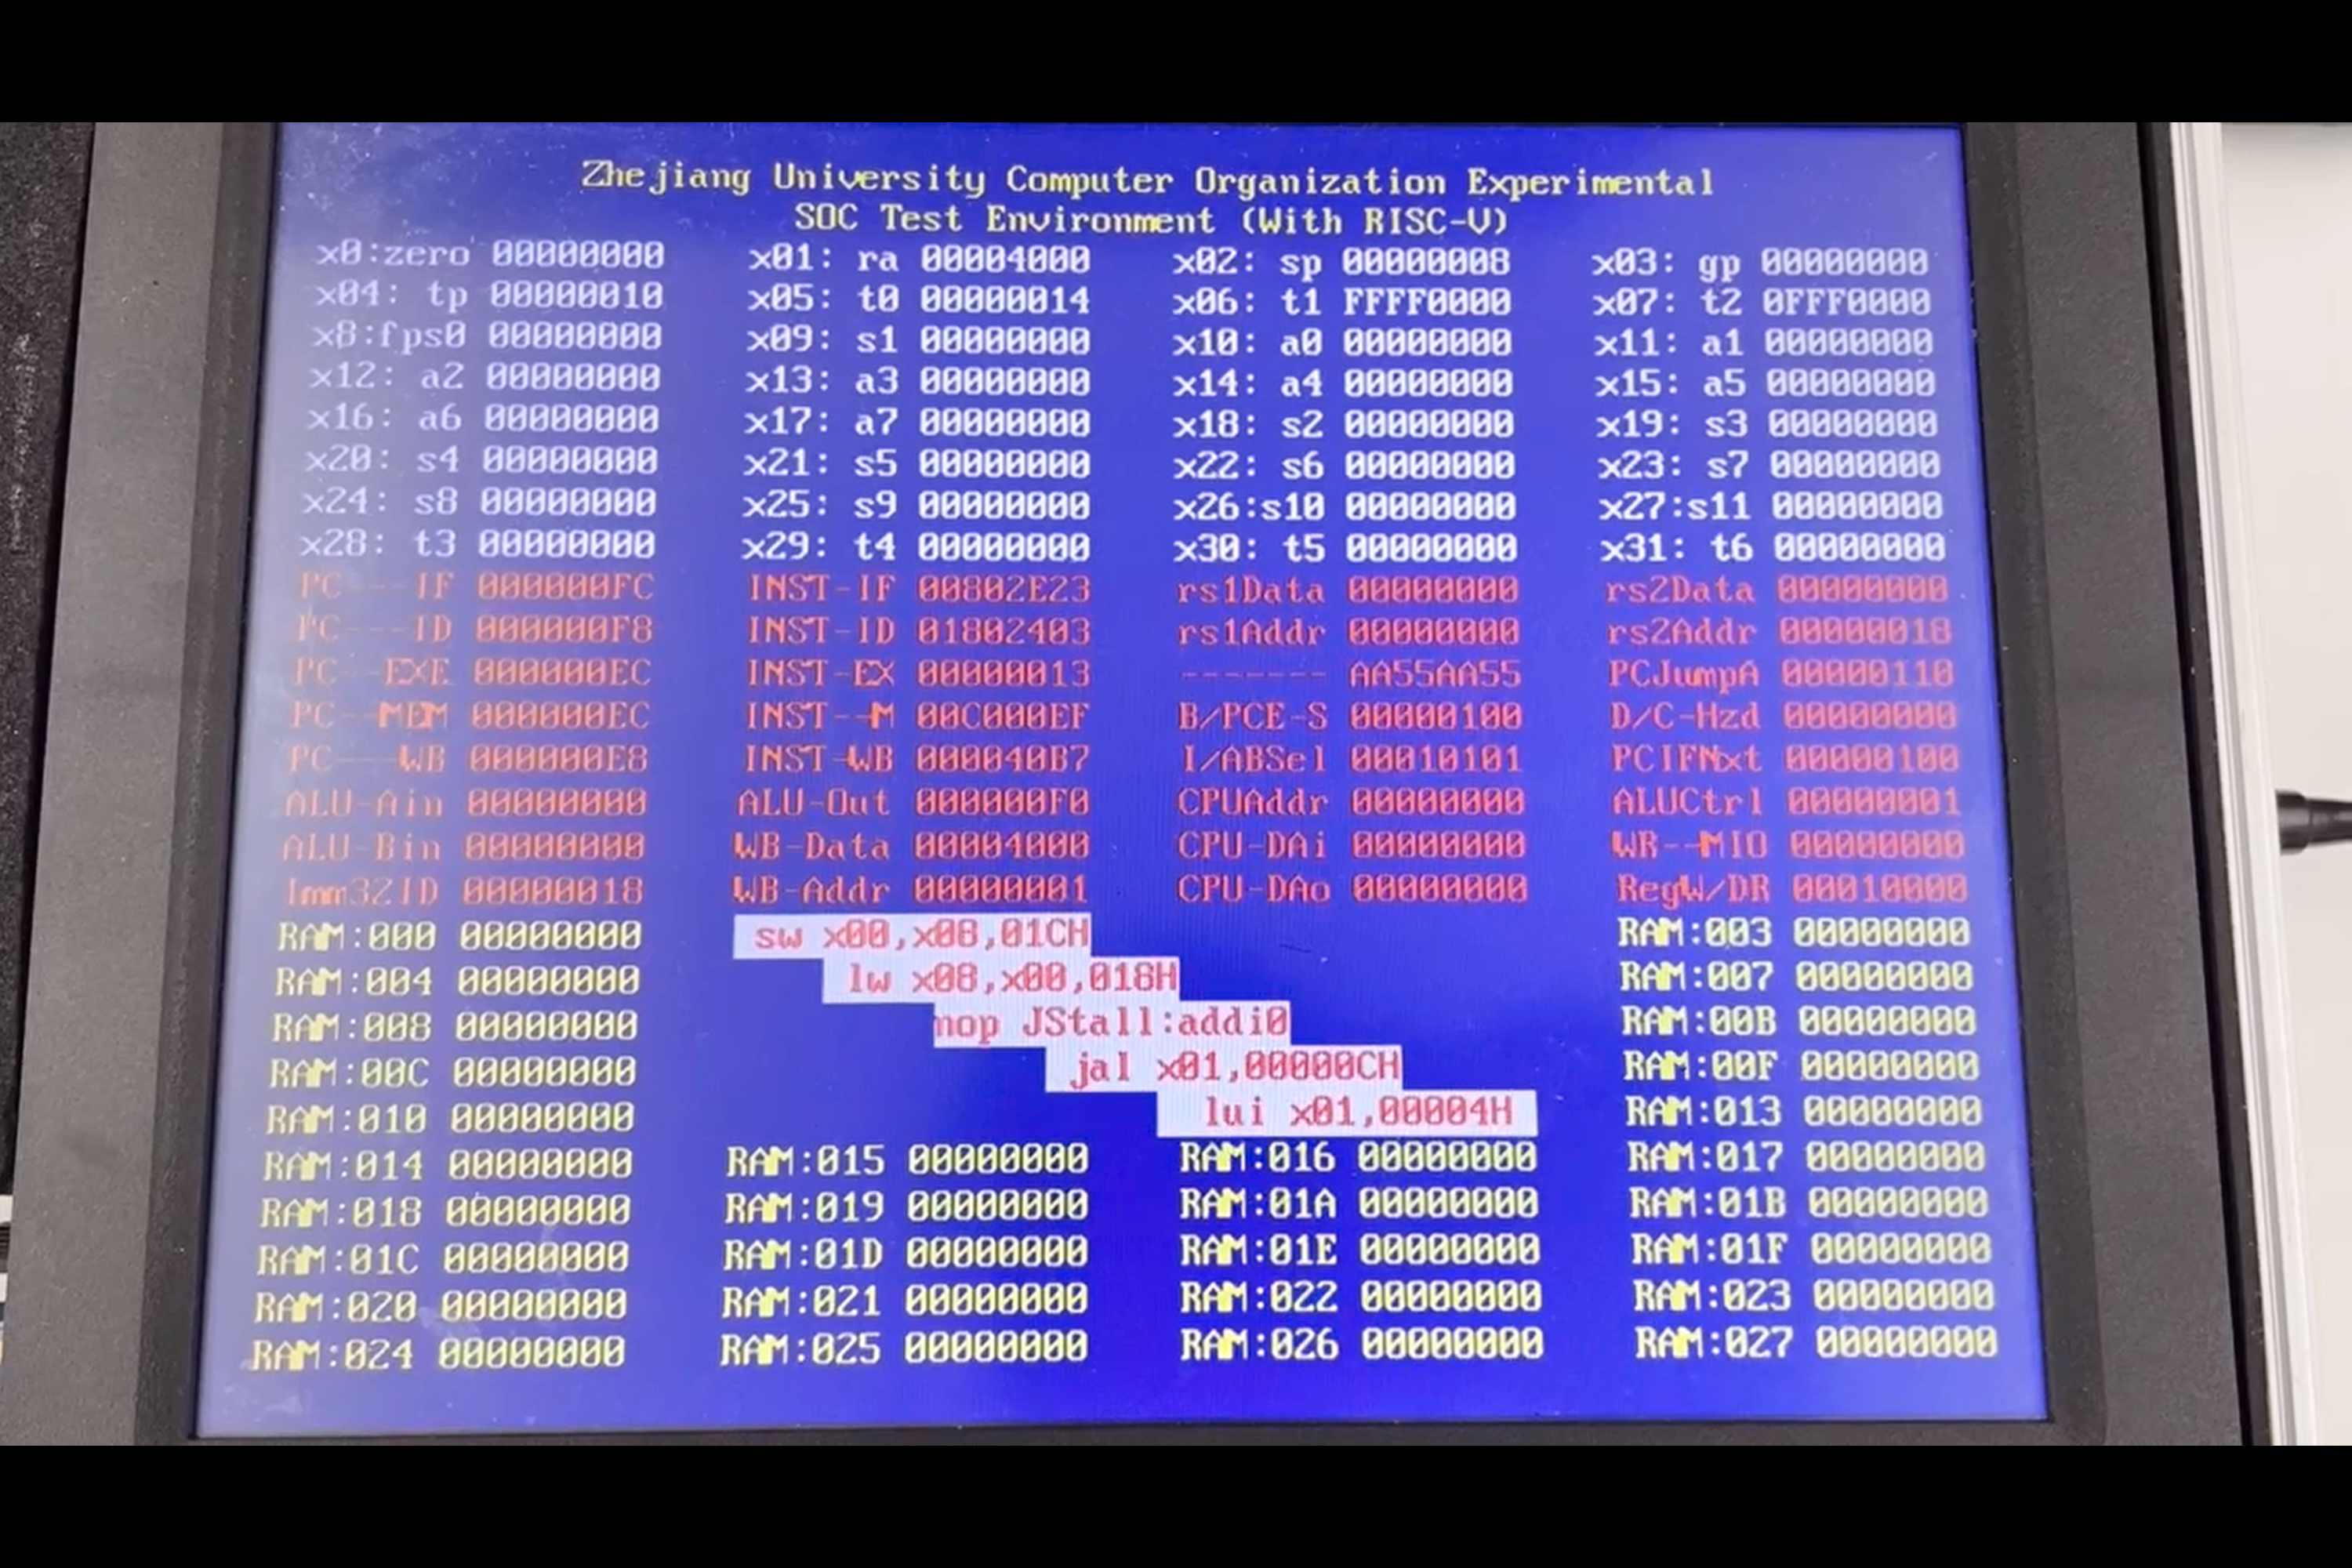
\includegraphics[width=1.0\textwidth]{y4.png} %插入图片,[]中设置图片大小,{}中是图片文件名
	\caption{验证结果图} %最终文档中希望显示的图片标题
	\label{Fig.10} %用于文内引用的标签
\end{figure}
\subsection{jalr指令检验}
\begin{figure}
	\centering %图片居中
	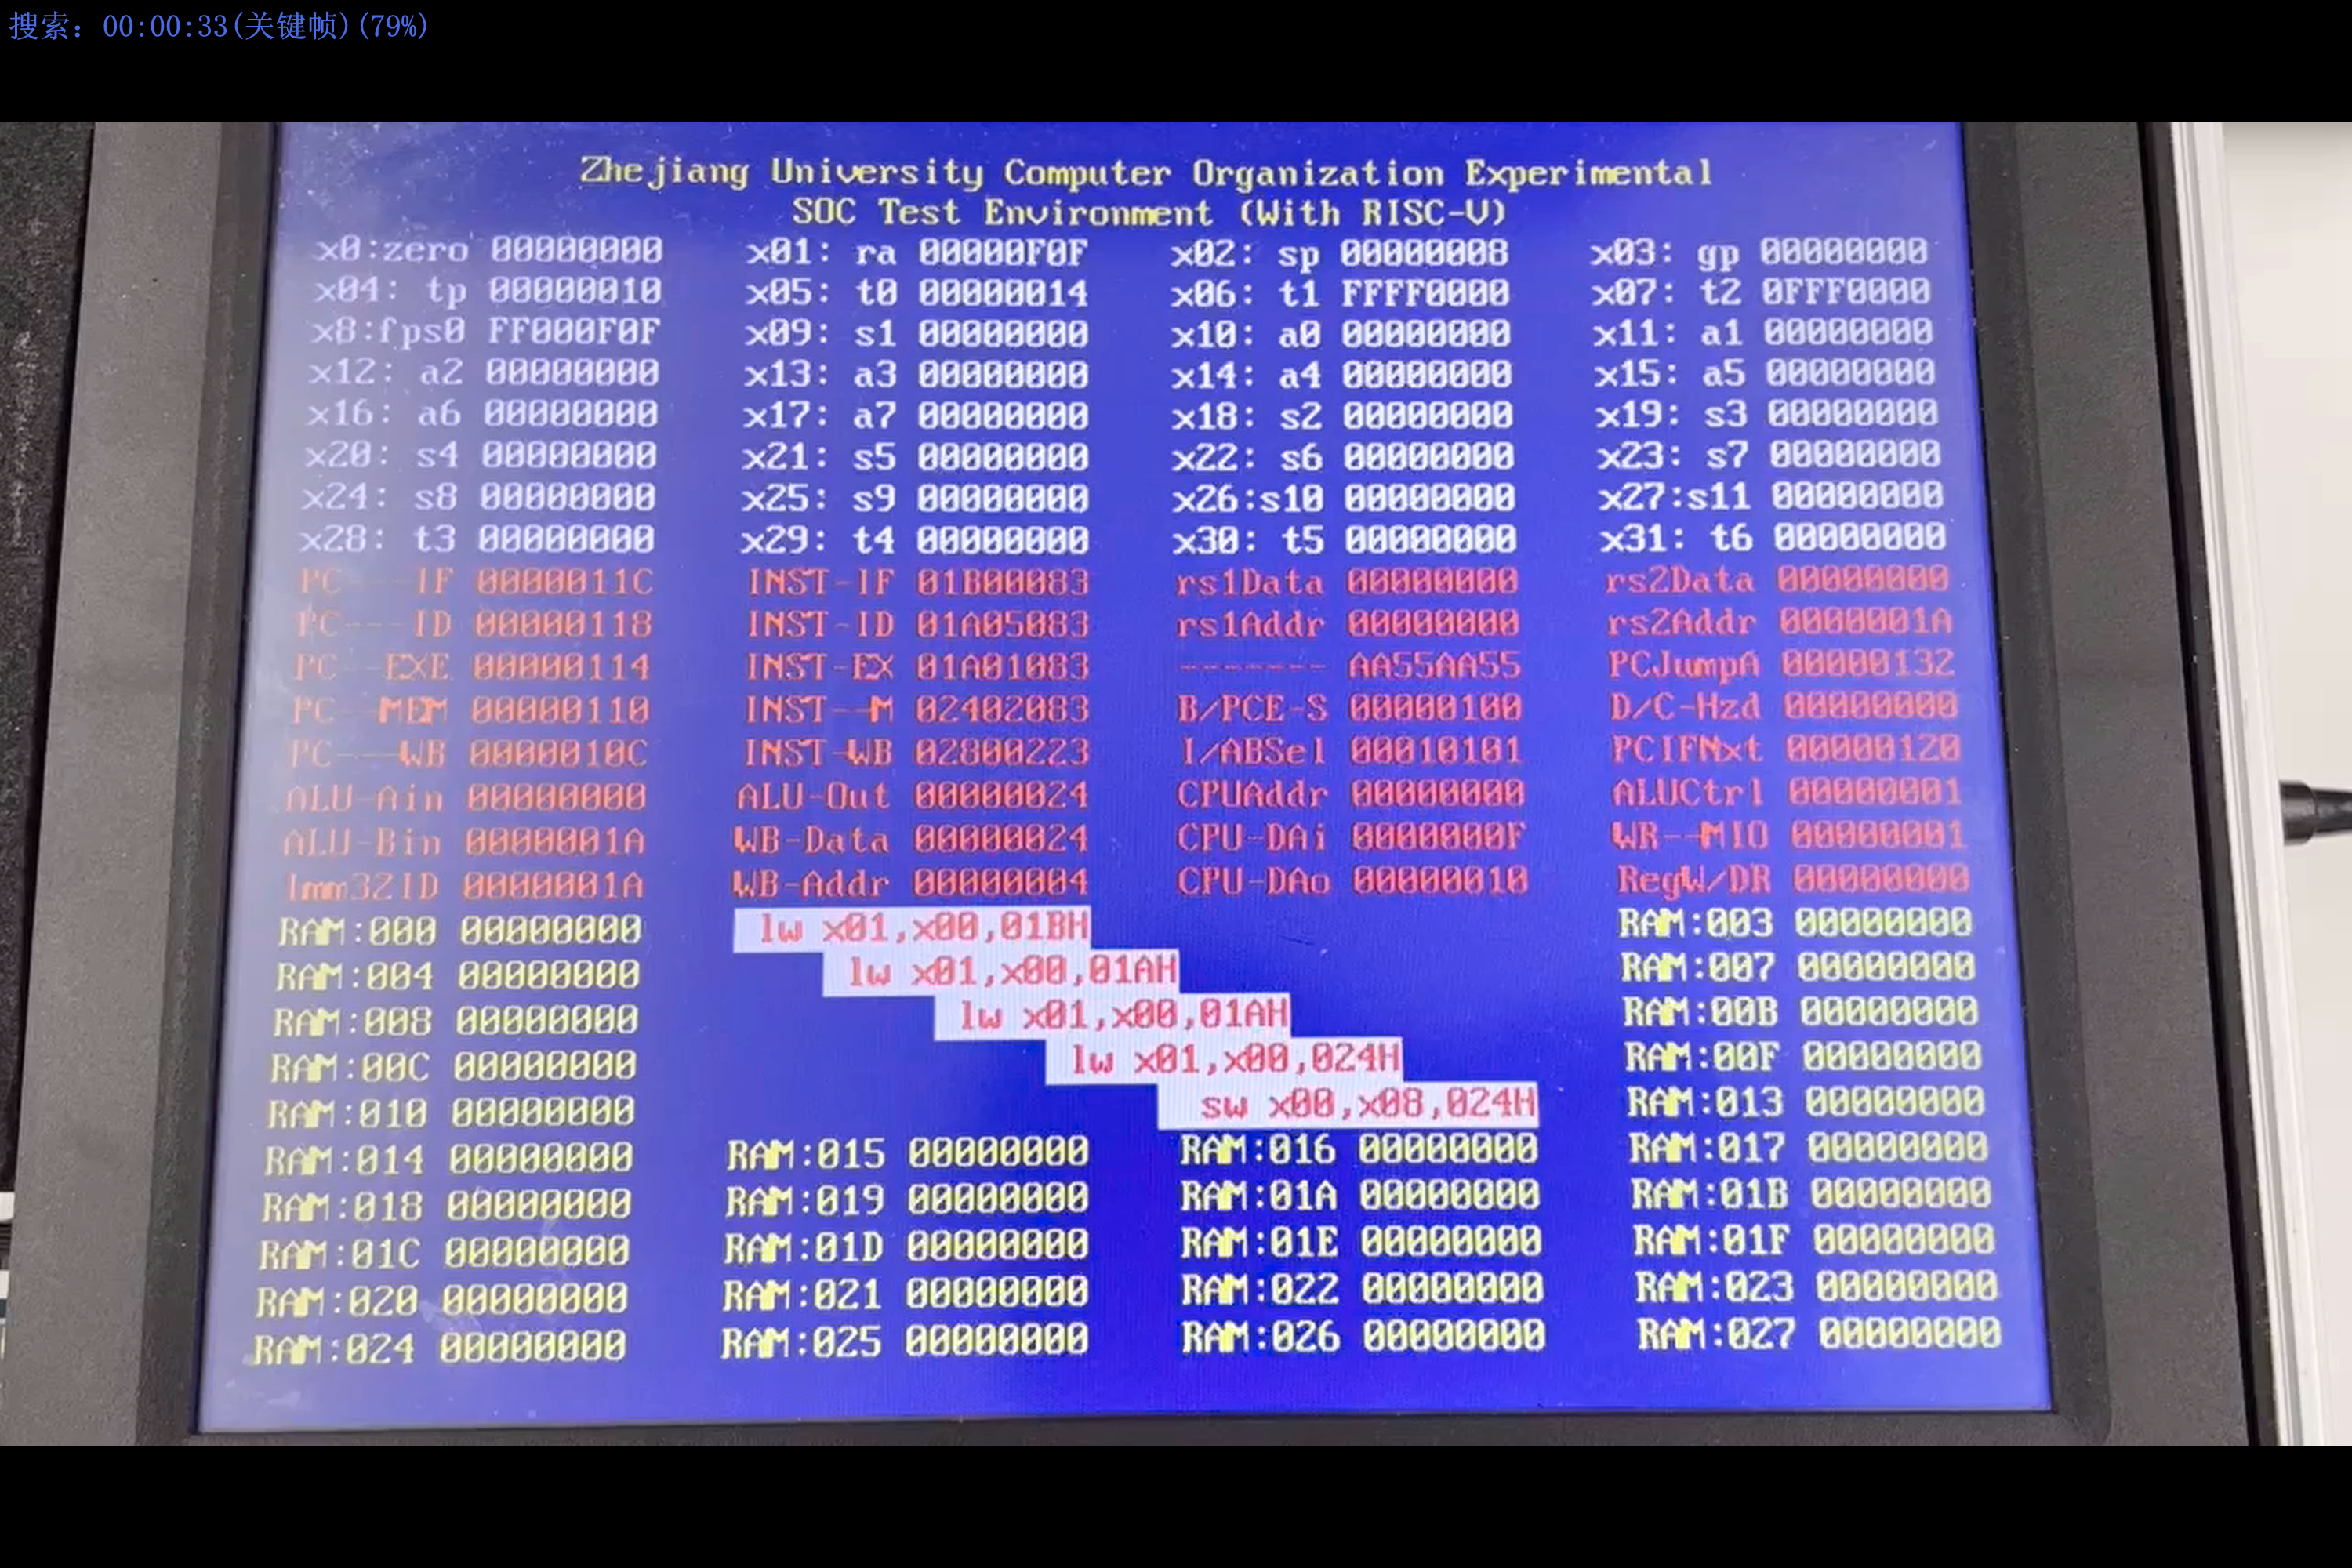
\includegraphics[width=1.0\textwidth]{y5.png} %插入图片,[]中设置图片大小,{}中是图片文件名
	\caption{验证结果图} %最终文档中希望显示的图片标题
	\label{Fig.11} %用于文内引用的标签
\end{figure}
最后,jalr指令跳回程序开头。见图4.12
\begin{figure}
	\centering %图片居中
	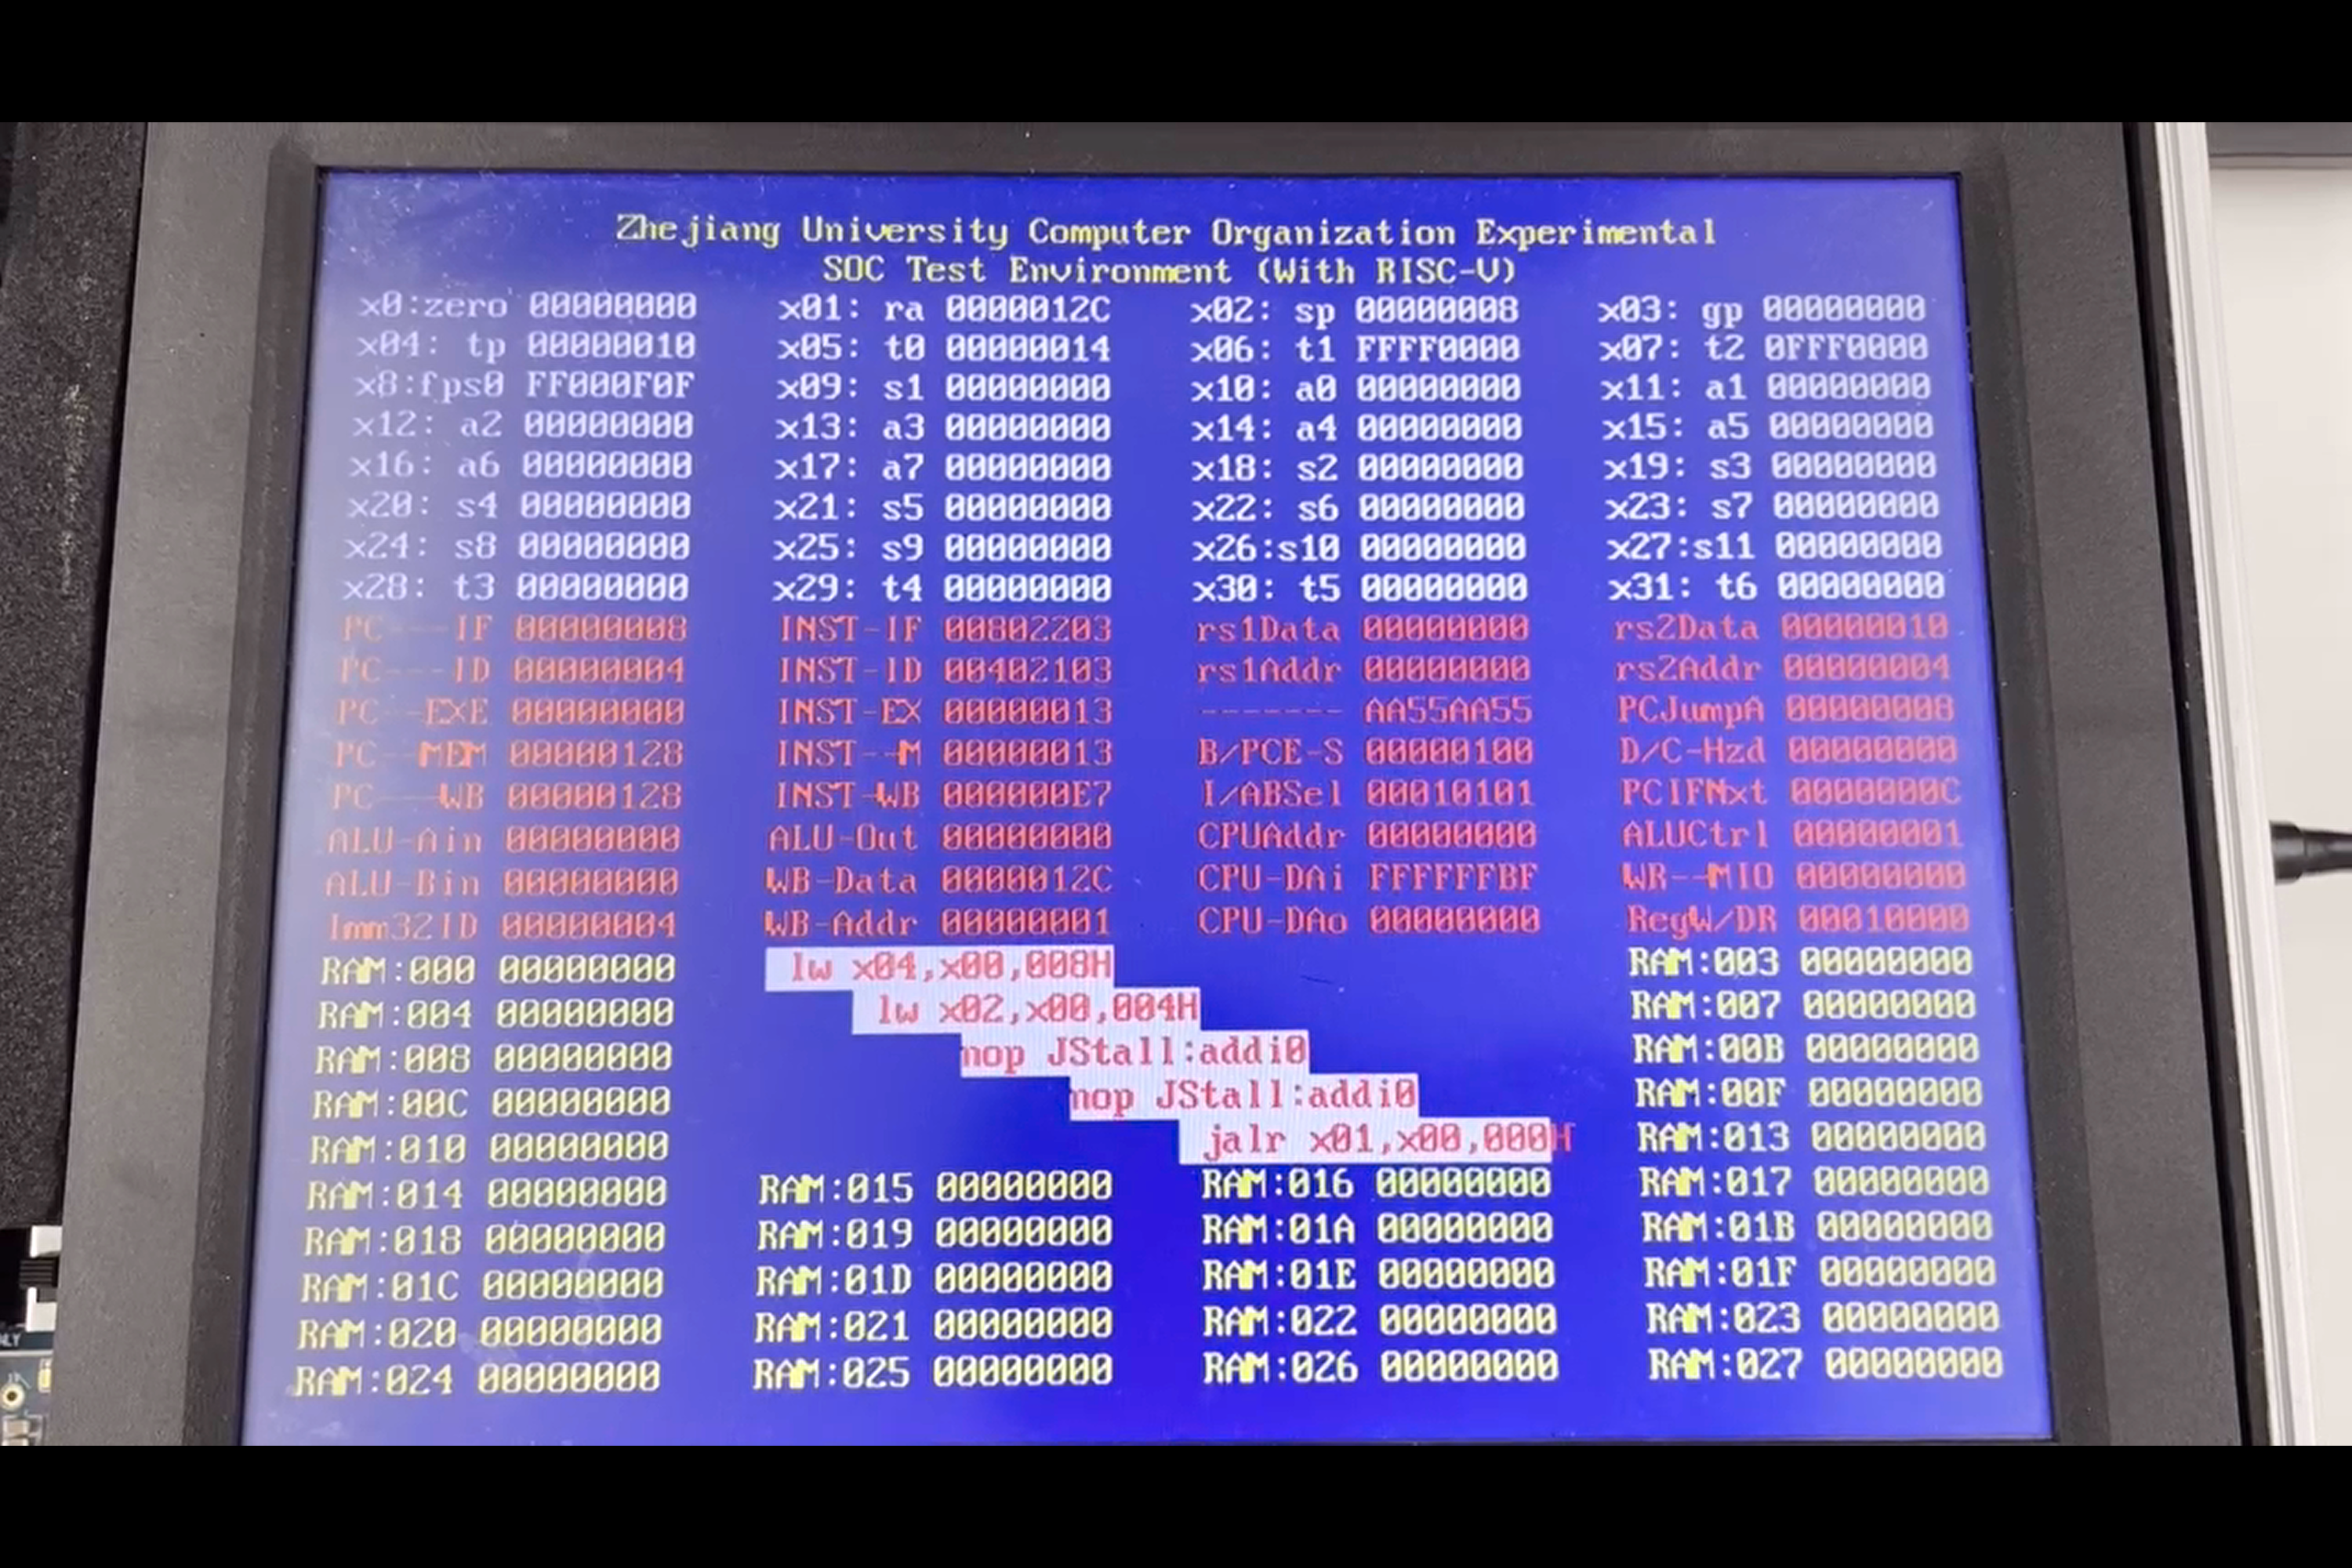
\includegraphics[width=1.0\textwidth]{y6.png} %插入图片,[]中设置图片大小,{}中是图片文件名
	\caption{验证结果图} %最终文档中希望显示的图片标题
	\label{Fig.12} %用于文内引用的标签
\end{figure}